\documentclass[12pt]{article}
\usepackage[a4paper,margin=2cm]{geometry}
\usepackage{newtxtext,newtxmath}
\usepackage{graphicx,booktabs,amsmath,url,xcolor,caption,subcaption,enumitem}
\usepackage[hidelinks]{hyperref}
\captionsetup{font=small,labelfont=bf,skip=3pt}
\setlist{nosep,leftmargin=*}
\setlength{\parskip}{2pt}
\setlength{\textfloatsep}{8pt}
\setlength{\floatsep}{6pt}
\setlength{\intextsep}{6pt}

\title{\vspace{-1.6cm}\textbf{Learning the Rhythm: Why Rotary Position Encoding Breaks Beyond the Training Horizon, and How Learnable Frequencies Fix It}}
\author{Liu Yuncong, Zhang Yihang, Ma Xiaoyu \quad {\normalsize(FT5011, National University of Singapore)}}
\date{\vspace{-0.9cm}}

\makeatletter\let\inputtab\@@input\makeatother
\begin{document}
\maketitle

\begin{abstract}\noindent
Forecasters in finance and energy need predictions at several horizons at once, yet a model is usually trained for one horizon.
A Transformer that represents each future step by a placeholder token, distinguished only by its rotary position encoding (RoPE), can in principle forecast any horizon.
With standard RoPE it does not: trained for 96 steps and asked for 720 (on hourly data, 4 days versus 30 days ahead), its error reaches up to 6 times that of a model trained for 720.
Our proposal's learnable time scale per attention head (4 parameters per layer) removes 38--66\% of this error, and we trace why: the learned scales tune RoPE's fastest rotation to the daily cycle, so unseen future positions look like positions seen in training.
Fixing the scale to the daily-aligned value, without learning, reproduces the gain; values 5\% off reproduce the failure.
The gain is significant (Diebold--Mariano) on strongly seasonal data, including two electricity markets, and absent on exchange rates, which have no cycle to align. Training on mixed horizons lets one model match per-horizon models.
\end{abstract}

\section{Problem and how we arrived at it}
Risk managers report Value-at-Risk at 1 and 10 days; energy traders bid for the next day and hedge the next week.
Maintaining one model per horizon is costly, so a model that is trained once and forecasts any horizon is useful --- for example, trained to forecast hourly electricity prices 4 days ahead and then asked for 30 days.
Our proposal asked whether a Transformer could \emph{learn} the time scales that matter, by giving each attention head a learnable multiplier on its rotary position frequencies.
On real data that hypothesis failed in its original form: the learned scales stayed within $\pm$10\% of 1, all heads learned nearly the same scale, and accuracy at the training horizon did not change.
However, the same scales made a large difference once we asked the model to forecast \emph{beyond} its training horizon.
This report explains where that effect appears (Sec.~4.2), what causes it (4.3), what does better (4.4), and what it means for financial data (Sec.~5).

\section{Model}
\textbf{Backbone.} Each univariate history of $L{=}336$ steps is cut into non-overlapping patches of $P{=}16$ steps, projected to $d{=}64$ dimensions, and processed by a 2-layer, 4-head pre-norm Transformer encoder.
After the 21 history tokens we append one learnable placeholder token per future patch (6 for $H{=}96$, 45 for $H{=}720$); all placeholders share the same vector, so \emph{only their position encodings tell them apart}.
History tokens attend to history only; each placeholder attends to all history and to itself, so the forecast for step $h$ does not depend on the total horizon and the model can be queried at any $H$ after training.
A shared linear layer reads each placeholder out into $P$ forecast values.
The structure follows the repository we started from; we chose patches because point tokens (Sec.~6) gave much noisier extrapolation.

\textbf{Rotary position encoding.} RoPE \cite{su2021roformer} rotates each pair $j$ of query/key coordinates at token position $t$ by the angle $t\,\omega_j$ with $\omega_j=b^{-j/m}$, $m=d_h/2=8$, base $b\in\{10^3,10^4\}$.
Because $\langle R(t\omega)q, R(u\omega)k\rangle$ depends only on $t-u$, attention sees relative distances.
The fastest pair rotates at $\omega_0=1$ rad/token, i.e.\ it repeats every $2\pi\approx6.28$ tokens.

\textbf{Learnable frequency scale (main method).} Each layer $\ell$ and head $h$ has a scalar $a_{\ell,h}$, initialised to 0, and uses $\hat\omega_{\ell,h,j}=\omega_j\,e^{a_{\ell,h}}$; this adds 4 parameters per layer and starts exactly at standard RoPE.
\emph{Variants} used as ablations: \emph{grouped} (separate scales for the 4 fastest and 4 slowest pairs), \emph{shared} (one scale per layer for all heads), and \emph{fixed} scales set by hand and not trained.

\textbf{Why alignment should matter.} If a series repeats every $T$ tokens and $\hat\omega_0=2\pi/T$, then position $t+T$ has exactly the same fastest-pair angle as $t$: a placeholder far beyond the training horizon is, to that pair, indistinguishable from one at the same time of day inside it.
With the default $\omega_0=1$ and, e.g., ETTm1 ($T=6$ tokens $=1$ day), the angle drifts by $0.28$ tokens per day and the model meets angle combinations it never saw.

\textbf{Multi-horizon training.} As a second remedy, each training batch uses a horizon drawn from $\{96,192,336,720\}$, so one model sees distant placeholders during training.

\section{Data, protocol and baselines}
\textbf{Data} (sources and URLs in Appendix B). Four standard benchmarks --- Electricity (321 clients, hourly), ETTh1/ETTm1 (transformer load, hourly/15-min), Weather (21 variables, 10-min) --- and three financial markets: day-ahead electricity prices of Nord Pool (EPF-NP) and PJM (EPF-PJM), hourly 2013--2018, and daily exchange rates of 8 currencies.
A \emph{step} is one observation. Following the long-term forecasting benchmarks \cite{zeng2023dlinear,nie2023patchtst}, models read $L{=}336$ past steps and forecast $H\in\{96,192,336,720\}$ steps; we train at $H{=}96$ and test up to 720. In calendar time, 96$\to$720 steps is 4$\to$30 days on hourly data (Electricity, ETTh1, EPF), 1$\to$7.5 days on ETTm1 and 16 h$\to$5 days on Weather; on daily exchange rates 720 steps ($\approx$3 years) exceeds any practical horizon and is kept only for a uniform protocol. Every variable is forecast as its own series. Splits are chronological (ETT: 12/4/4 months; others 70/10/20\%); z-scores use training rows only; for exchange rates we add per-window normalisation (RevIN), without which every model fails on this drifting series.
We report MSE on the normalised scale.

\textbf{Protocol.} All models share the backbone, optimiser (AdamW, lr $10^{-3}$, warm-up + cosine), batch order, initial weights (paired seeds) and a fixed step budget per dataset.
The RoPE base and the best checkpoint are chosen on the validation set only; the test set is used once. We use 3 seeds (5 on ETTh1 ablations).

\textbf{Baselines and why.} (i) \emph{Fixed RoPE}, the same model without the scales, isolates the mechanism; (ii) a channel-wise \emph{linear} model $\mathbb{R}^{336}\!\to\!\mathbb{R}^{H}$, because simple linear models match Transformers on these benchmarks \cite{zeng2023dlinear}; (iii) models \emph{trained directly} at $H{=}720$, the natural alternative to extrapolation.

\textbf{Significance.} Beyond mean $\pm$ std over seeds, we run a Diebold--Mariano test \cite{diebold1995} per seed and base on the per-origin loss difference fixed$-$learnable (steps 97--720), with a Newey--West variance (lag 719) for overlapping windows.

\section{Results}
\subsection{At the training horizon the model is competitive, and the scales change nothing}
\begin{table}[h]\centering\small
\caption{Train and test MSE at the training horizon $H{=}96$ (mean$\pm$std over seeds). Published PatchTST test MSE for reference: Electricity 0.129, ETTh1 0.370, ETTm1 0.290, Weather 0.149 \cite{nie2023patchtst}.}
\label{tab:in}
\begin{tabular}{lcccccc}\toprule
& \multicolumn{2}{c}{Linear} & \multicolumn{2}{c}{Transformer, fixed RoPE} & \multicolumn{2}{c}{Transformer, learnable scale}\\
\cmidrule(lr){2-3}\cmidrule(lr){4-5}\cmidrule(lr){6-7}
Dataset & train & test & train & test & train & test\\\midrule
\inputtab tables/t1_inhorizon.tex 
\bottomrule\end{tabular}\end{table}
The Transformer is close to published results; it beats the linear model clearly on Weather and EPF-NP, ties on Electricity, and loses on ETTh1, ETTm1 and exchange rates, in line with \cite{zeng2023dlinear}.
Learnable scales neither help nor hurt at $H{=}96$. Weather's lower test than train error reflects a calmer test period, not leakage.

\subsection{Beyond the training horizon, fixed RoPE collapses and learnable scales prevent it}
\begin{figure}[h]\centering
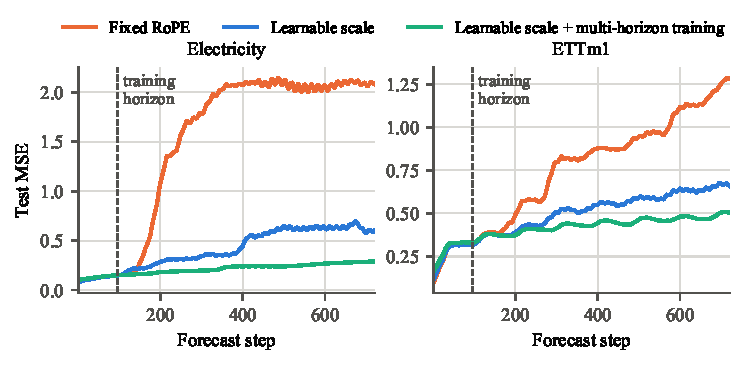
\includegraphics{figures/fig1_perstep.pdf}
\caption{Test MSE per forecast step for models trained at $H{=}96$ (base $10^4$, mean of 3 seeds). Fixed RoPE degrades as soon as it leaves the training horizon.}
\label{fig:perstep}\end{figure}
\begin{table}[h]\centering\small
\caption{Test MSE over steps 1--720. Columns 2--3: trained at $H{=}96$ and queried at 720. DM: of 6 runs (seed$\times$base), how many are significantly better\,/\,worse with learnable scales ($p{<}0.05$). Columns 5--7: one multi-horizon model, and models trained directly at 720.}
\label{tab:ex}
\begin{tabular}{lcccccc}\toprule
& \multicolumn{2}{c}{Trained at 96} & DM & Multi-horizon & \multicolumn{2}{c}{Trained at 720}\\
\cmidrule(lr){2-3}\cmidrule(lr){6-7}
Dataset & fixed & learnable & +\,/\,$-$ & learnable & Transformer & Linear\\\midrule
\inputtab tables/t2_extrap.tex 
\bottomrule\end{tabular}\end{table}
Figure~\ref{fig:perstep} and Table~\ref{tab:ex} show the central finding. Queried at 720 steps, fixed RoPE reaches 1.5--6.4 times the error of a Transformer trained at 720 on Electricity, ETTh1 and ETTm1; the learnable scale cuts its error by 38--66\%, significantly in every run on these datasets.
On ETTh1, the extrapolating model even beats every model trained directly at 720, which overfit this small dataset.

\subsection{Why: the learned scales align RoPE with the daily cycle}
\begin{figure}[h]
\begin{minipage}[t]{0.50\linewidth}\centering\small
\captionof{table}{Mechanism ablations, all trained at $H{=}96$ (test MSE).}\label{tab:mech}
\begin{tabular}{@{}lc@{}}\toprule
Frequency scales & Test MSE\\\midrule
\inputtab tables/t3_mechanism.tex 
\bottomrule\end{tabular}
\end{minipage}\hfill
\begin{minipage}[t]{0.47\linewidth}\centering
\vspace{0pt}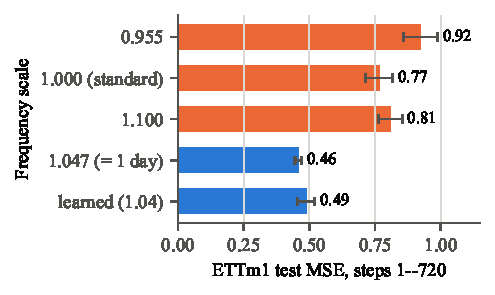
\includegraphics[width=\linewidth]{figures/fig2_alignment.pdf}
\captionof{figure}{ETTm1, 6 tokens per day: scale $2\pi/6=1.047$ aligns RoPE's fastest rotation with the day. Fixed at 1.047 without learning it matches the learned model; 5\% too slow or fast collapses like standard RoPE.}\label{fig:align}
\end{minipage}
\end{figure}
Four observations point to one cause.
\textbf{(1) Learning, not diversity, matters.} Sharing one scale across heads is as good as one per head, and hand-set spreads of head scales help little or not at all (Table~\ref{tab:mech}); so the proposal's picture of heads specialising to time scales is not what happens.
\textbf{(2) Only the fast frequencies matter.} In the grouped variant the fast group learns the same value as the per-head scale, while the slow group drifts freely (0.95--1.13) with no effect on the forecast.
\textbf{(3) The learned value is the aligning value.} On ETTm1 one day is 6 tokens, and the learned scales average 1.04 against the aligning $2\pi/6=1.047$. Fixing 1.047 reproduces the gain with no learning; 0.955 or 1.10 reproduce the collapse (Fig.~\ref{fig:align}; DM $p<10^{-10}$ in all six runs).
\textbf{(4) The more seasonal a series, the larger the gain} (Fig.~\ref{fig:season}). Across channels the ratio fixed/learnable rises with daily seasonal strength \cite{wang2006}: on ETTm1 fixed RoPE's error is 1.8 times the learnable model's on the two most seasonal load channels, and in Weather only the three solar-radiation channels gain (ratio 1.14--1.17); the other 18 Weather variables have no gain, which is why Weather as a whole shows none.
Across datasets the relation is clear at the extremes (Electricity largest, exchange rates none) but loose in between (EPF-PJM gains more than its seasonal strength suggests), so seasonal strength indicates where to expect a gain but does not predict its size.
Attention confirms the picture: on ETTm1 the share of placeholder attention on history patches at the same time of day stays at 0.53 for all 7.5 days ahead with scale 1.047, but with fixed RoPE falls from 0.64 to 0.05, below the chance level of 1/6, after two days. We also ruled out gradient clipping (inactive after warm-up).
\begin{figure}[h]\centering
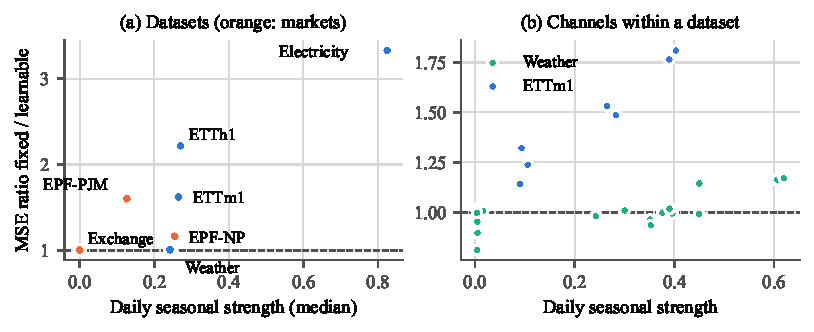
\includegraphics{figures/fig3_periodicity.pdf}
\caption{Gain from learnable scales (MSE ratio fixed/learnable on steps 97--720; $>1$ means learnable is better) against daily seasonal strength.}
\label{fig:season}\end{figure}

\subsection{How far it goes: multi-horizon training}
Aligning the fastest frequency fixes the phase but not everything: on Electricity, ETTm1 and Weather the extrapolating model stays above models trained at 720 (Table~\ref{tab:ex}).
A single model trained on mixed horizons is within 3\% of, or better than, the Transformer trained at 720 on all seven datasets, at a small cost at $H{=}96$ (Electricity 0.135 vs 0.128 on the same windows); with it, fixed and learnable RoPE perform alike, because distant positions are no longer unseen.
Multi-horizon training is therefore the stronger remedy when long training targets exist; learnable scales are the remedy when they do not, or when long-horizon training overfits (ETTh1, EPF-NP).

\section{Application to finance}
Our results give a concrete rule for financial forecasting: \emph{position encodings must be aligned with the calendar cycle of the series, and learnable RoPE scales do this automatically.}
We tested this on financial data chosen before seeing results. Electricity prices are traded assets with strong daily cycles; on both markets learnable scales reduce 720-step error significantly (EPF-PJM 0.44$\to$0.27, significant in 6/6 runs; EPF-NP 1.07$\to$0.90, 5/6).
Exchange rates behave like a random walk with no cycle; here the scales have no consistent effect (3 runs significantly better, 3 worse), the linear model is best, and RevIN is essential --- as the mechanism predicts.
In practice: (i) for seasonal financial series --- intraday volume and volatility (daily U-shape), power and gas prices --- use learnable or calendar-aligned RoPE before forecasting beyond the training horizon; (ii) to cover several risk horizons (1- and 10-day VaR, daily-to-weekly volatility as in HAR) with one model, train on mixed horizons; (iii) for near-random-walk prices, position encodings will not help.

\section{Limitations and conclusion}
Heads did not specialise to distinct time scales, as the proposal expected, and grouping frequencies did not help. The model is small and seeds are few (partly offset by DM tests); with point tokens the effect is noisier; linear models stay strong at the training horizon.
In short, RoPE fails beyond the training horizon because its rotation is out of step with the data's daily rhythm; four learnable parameters per layer fix the phase, and mixed-horizon training closes the remaining gap.

\begingroup\small
\begin{thebibliography}{9}\setlength{\itemsep}{0pt}
\bibitem{su2021roformer} J. Su et al. RoFormer: Enhanced Transformer with rotary position embedding. arXiv:2104.09864, 2021.
\bibitem{zeng2023dlinear} A. Zeng, M. Chen, L. Zhang, Q. Xu. Are Transformers effective for time series forecasting? AAAI 2023.
\bibitem{nie2023patchtst} Y. Nie et al. A time series is worth 64 words: long-term forecasting with Transformers. ICLR 2023.
\bibitem{diebold1995} F. X. Diebold, R. S. Mariano. Comparing predictive accuracy. J. Business \& Economic Statistics, 1995.
\bibitem{wang2006} X. Wang, K. Smith, R. Hyndman. Characteristic-based clustering for time series data. Data Mining and Knowledge Discovery, 2006.
\bibitem{lago2021} J. Lago, G. Marcjasz, B. De Schutter, R. Weron. Forecasting day-ahead electricity prices: a review of state-of-the-art algorithms, best practices and an open-access benchmark. Applied Energy, 2021.
\end{thebibliography}
\endgroup

\clearpage
\appendix
\section*{Appendix A. Step-by-step replication}
All runs used Python 3.13, PyTorch 2.6 (CUDA 12.4) on one NVIDIA H100 (memory capped at 8\%); a run takes 20 s--3 min. Code: repository \url{https://github.com/ycsama0703/ft5011-ropeformer} plus the scripts in \texttt{experiments/}.
\begin{enumerate}
\item \texttt{pip install -e .} (PyTorch $\ge$2.0); \texttt{python -m unittest discover -s tests} (29 tests).
\item Data: \texttt{python tools/download\_data.py ETTh1 ETTm1 weather electricity exchange\_rate}; financial data: \texttt{python experiments/build\_fin.py raw data} after downloading EPF (Appendix B).
\item Train at 96 and extrapolate, with direct-training references, for each dataset $D$ and its step budget $S$ (ETTh1, EPF, exchange: 2000; ETTm1: 4000; Weather: 6000; Electricity: 8000):\\
\texttt{python tools/extrap\_study.py --dataset D --steps S --patch-len 16 --amp bf16 --seeds 0 1 2 --bases 1000 10000 --modes standard head grouped --eval-horizons 192 336 720 --direct-horizons 336 720 --direct-modes head --out results/r2\_D.json} (add \texttt{--instance-norm} for exchange rates).
\item Multi-horizon: \texttt{python tools/multi\_horizon.py --dataset D --steps S --train-horizons 96 192 336 720 --test-horizon 720 --out results/mh\_D.json}.
\item Ablations (Table~\ref{tab:mech}): \texttt{extrap\_study.py} with \texttt{--modes shared\_group fixed\_head:0.9,0.97,1.03,1.1 fixed\_head:0.5,0.8,1.25,2.0} (ETTh1, 5 seeds) and \texttt{fixed\_head:1.0472,1.0472,1.0472,1.0472} etc.\ (ETTm1).
\item Train/val/test MSE at 96, linear reference, Diebold--Mariano tests, per-channel analysis and seasonal strength: scripts \texttt{train\_eval.py}, \texttt{linear96.py}, \texttt{dm\_test.py}, \texttt{per\_channel.py}, \texttt{periodicity.py} in \texttt{experiments/} (commands in \texttt{experiments/README.md}).
\item All tables and figures of this report: \texttt{python report/make\_assets.py}.
\end{enumerate}
Hyper-parameters: $L{=}336$, patch 16, $d{=}64$, 4 heads, 2 layers, FFN 128, dropout 0.1, batch 256, AdamW (lr $10^{-3}$, weight decay 0.01, none on scales), 300 warm-up steps then cosine decay, gradient clip 1.0, bf16 autocast; validation every 200--500 steps keeps the best state.

\section*{Appendix B. Data sources}
\begin{itemize}
\item ETTh1, ETTm1, Weather, Electricity, exchange rates: Time-Series-Library collection (CC BY 4.0), \url{https://huggingface.co/datasets/thuml/Time-Series-Library}.
\item EPF day-ahead prices (Nord Pool, PJM; hourly 2013--2018) \cite{lago2021}: \url{https://zenodo.org/records/4624805} (files \texttt{NP.csv}, \texttt{PJM.csv}); we keep the price column only.
\item Bitcoin (supplementary, low seasonality): Binance public 1-hour klines, \url{https://data.binance.vision}, BTCUSDT 2019--2024; channels log volume, log trade count, $|$log return$|$.
\end{itemize}
\end{document}
